\documentclass{article}
\usepackage{graphicx}
\usepackage[utf8]{inputenc}
\usepackage[main=english,vietnamese]{babel}
\usepackage{amsmath}
\usepackage{hyperref}
\usepackage{amsthm}
\usepackage{tcolorbox}
\usepackage{amsfonts}
\usepackage{amssymb}
\usepackage{mathrsfs}
\usepackage{centernot}
\usepackage{cases}
\usepackage{physics}
\usepackage[shortlabels]{enumitem}
\usepackage{tikz}
\usepackage{lipsum}
\usepackage{biblatex}
\usepackage{sidecap}
\usepackage{verbatim}
\usepackage{listings}

\addbibresource{main.bib}

\usetikzlibrary{calc}
\usetikzlibrary{decorations.pathmorphing}

\definecolor{borderblue}{HTML}{33c2ff}
\definecolor{codegreen}{rgb}{0,0.6,0}
\definecolor{codegray}{rgb}{0.5,0.5,0.5}
\definecolor{codepurple}{rgb}{0.58,0,0.82}
\definecolor{backcolour}{rgb}{0.95,0.95,0.92}

\lstdefinestyle{mystyle}{
    backgroundcolor=\color{backcolour},   
    commentstyle=\color{codegreen},
    keywordstyle=\color{magenta},
    numberstyle=\tiny\color{codegray},
    stringstyle=\color{codepurple},
    basicstyle=\ttfamily\footnotesize,
    breakatwhitespace=false,         
    breaklines=true,                 
    captionpos=b,                    
    keepspaces=true,                 
    numbers=left,                    
    numbersep=5pt,                  
    showspaces=false,                
    showstringspaces=false,
    showtabs=false,
    tabsize=2
}

\lstset{style=mystyle}

\newcommand{\paren}[1]{\left(#1\right)}
\newcommand{\curly}[1]{\left\{#1\right\}}

\allowdisplaybreaks

\makeatletter
\long\def\paragraph{%
  \@startsection{paragraph}{4}%
  {\z@}{2ex \@plus 1ex \@minus .2ex}{-1em}%
  {\normalfont\normalsize\bfseries}%
}
\makeatother

\makeatletter
\def\@xequals@fill{\arrowfill@\Relbar\Relbar\Relbar}
\newcommand*\xequals[2][]{\DOTSB\ext@arrow0055\@xequals@fill{#1}{#2}}
\makeatother

\makeatletter
\renewcommand*\env@matrix[1][*\c@MaxMatrixCols c]{%
  \hskip -\arraycolsep
  \let\@ifnextchar\new@ifnextchar
  \array{#1}}
\makeatother

\NewTColorBox{algorithm}{m}{
  standard jigsaw,
  sharp corners,
  boxrule=0.4pt,
  coltitle=black,
  colframe=black,
  opacityback=0,
  opacitybacktitle=0,
  fonttitle=\normalfont\bfseries\upshape,
  fontupper=\normalfont,
  title={Algorithm #1},
  after title={.},
  attach title to upper={\ },
}

\NewTColorBox{question}{m}{
  standard jigsaw,
  sharp corners,
  boxrule=0.4pt,
  coltitle=black,
  colframe=black,
  opacityback=0,
  opacitybacktitle=0,
  fonttitle=\normalfont\bfseries\upshape,
  fontupper=\normalfont,
  title={Question #1},
  attach title to upper={\ },
}

\title{R-Trees}
\author{\textbf{Group 6: ARR-CHEESE}\\\foreignlanguage{vietnamese}{Trần Tôn Minh Kỳ, Phan Anh Khoa, Lê Lương Quốc Trung,}\\\foreignlanguage{vietnamese}{Phạm Võ Khang Duy}}
\date{March 2025}

\begin{document}

\maketitle

\begin{abstract}
    Spatial data indexing requires multidimensional queries and modifications. The R-Tree, proposed by Antonin Guttman in 1984, attempts to solve this dilemma with worst case linearithmic time complexity. Due to the robust implementation on main memory and disk, it is extremely practical in real world applications and opens the door to additional variants in an attempt to counter technical issue the traditional R-Tree suffers from.
\end{abstract}

\tableofcontents

\newpage
\section{Introduction}
Spatial data structures present a rather different challenge from those of one-dimensional. Suppose that we wish to seek a restaurant's $xy$ coordinates. One may propose that we index the $x$-coordinate and $y$-coordinate in separate data structures and thus perform basic operations on one of them at a time. Because the search space is multi-dimensional, traditional one-dimensional data structures such as BSTs, B-trees are not well-suited for these purposes \cite{Guttman1984}. Thus the dilemma requires storing spatial attributes that can efficiently answers multidimensional queries. To this end, we present the R-Tree.

In the succeeding section, the first \textbf{Subsection 2.1} will introduce what is an R-Tree and its general implementation. \textbf{Subsection 2.2} and \textbf{2.3} will delve deeper into its implementation; the former will outline them in pseudocode and the latter will realize that outline using C++. \textbf{Subsection 2.4} will analyze the spacetime complexity of our implementations, whereas \textbf{Subsection 2.5} will dive in the practical purposes of R-Tree. \textbf{Subsection 2.6} will conclude this report with a few drawbacks of R-Tree and some other variants of R-Trees.

\section{R-Trees}
\subsection{Definitions}
An R-Tree is a height-balanced tree similar to a B-Tree \cite{Guttman1984} (all nodes remain sorted and all operations are in logarithmic time). R-Trees cater to spatial objects such as coordinates and thus points, rectangles, polygons, etc. As such, it is a suitable data structure to index objects in main memory and secondary storage. It is also capable of storing a multitude of data types using a concept known as Minimum Bounding Rectangle (henceforth will be referred to as MBRs) \cite{Papadopoulos2018}.

The R-Tree nodes are implemented as disk pages, where each node is an MBR bounding its children. The leaf nodes are pointers to the objects being indexed (indeed, the MBRs can overlap and contain multiple nodes). It should be noted that each MBR corresponds to each nodes and thus a search query requires traversing through many nodes before reaching its target node, if one exists in the first place \cite{Manolopoulos2006}.

\begin{figure}[ht]
	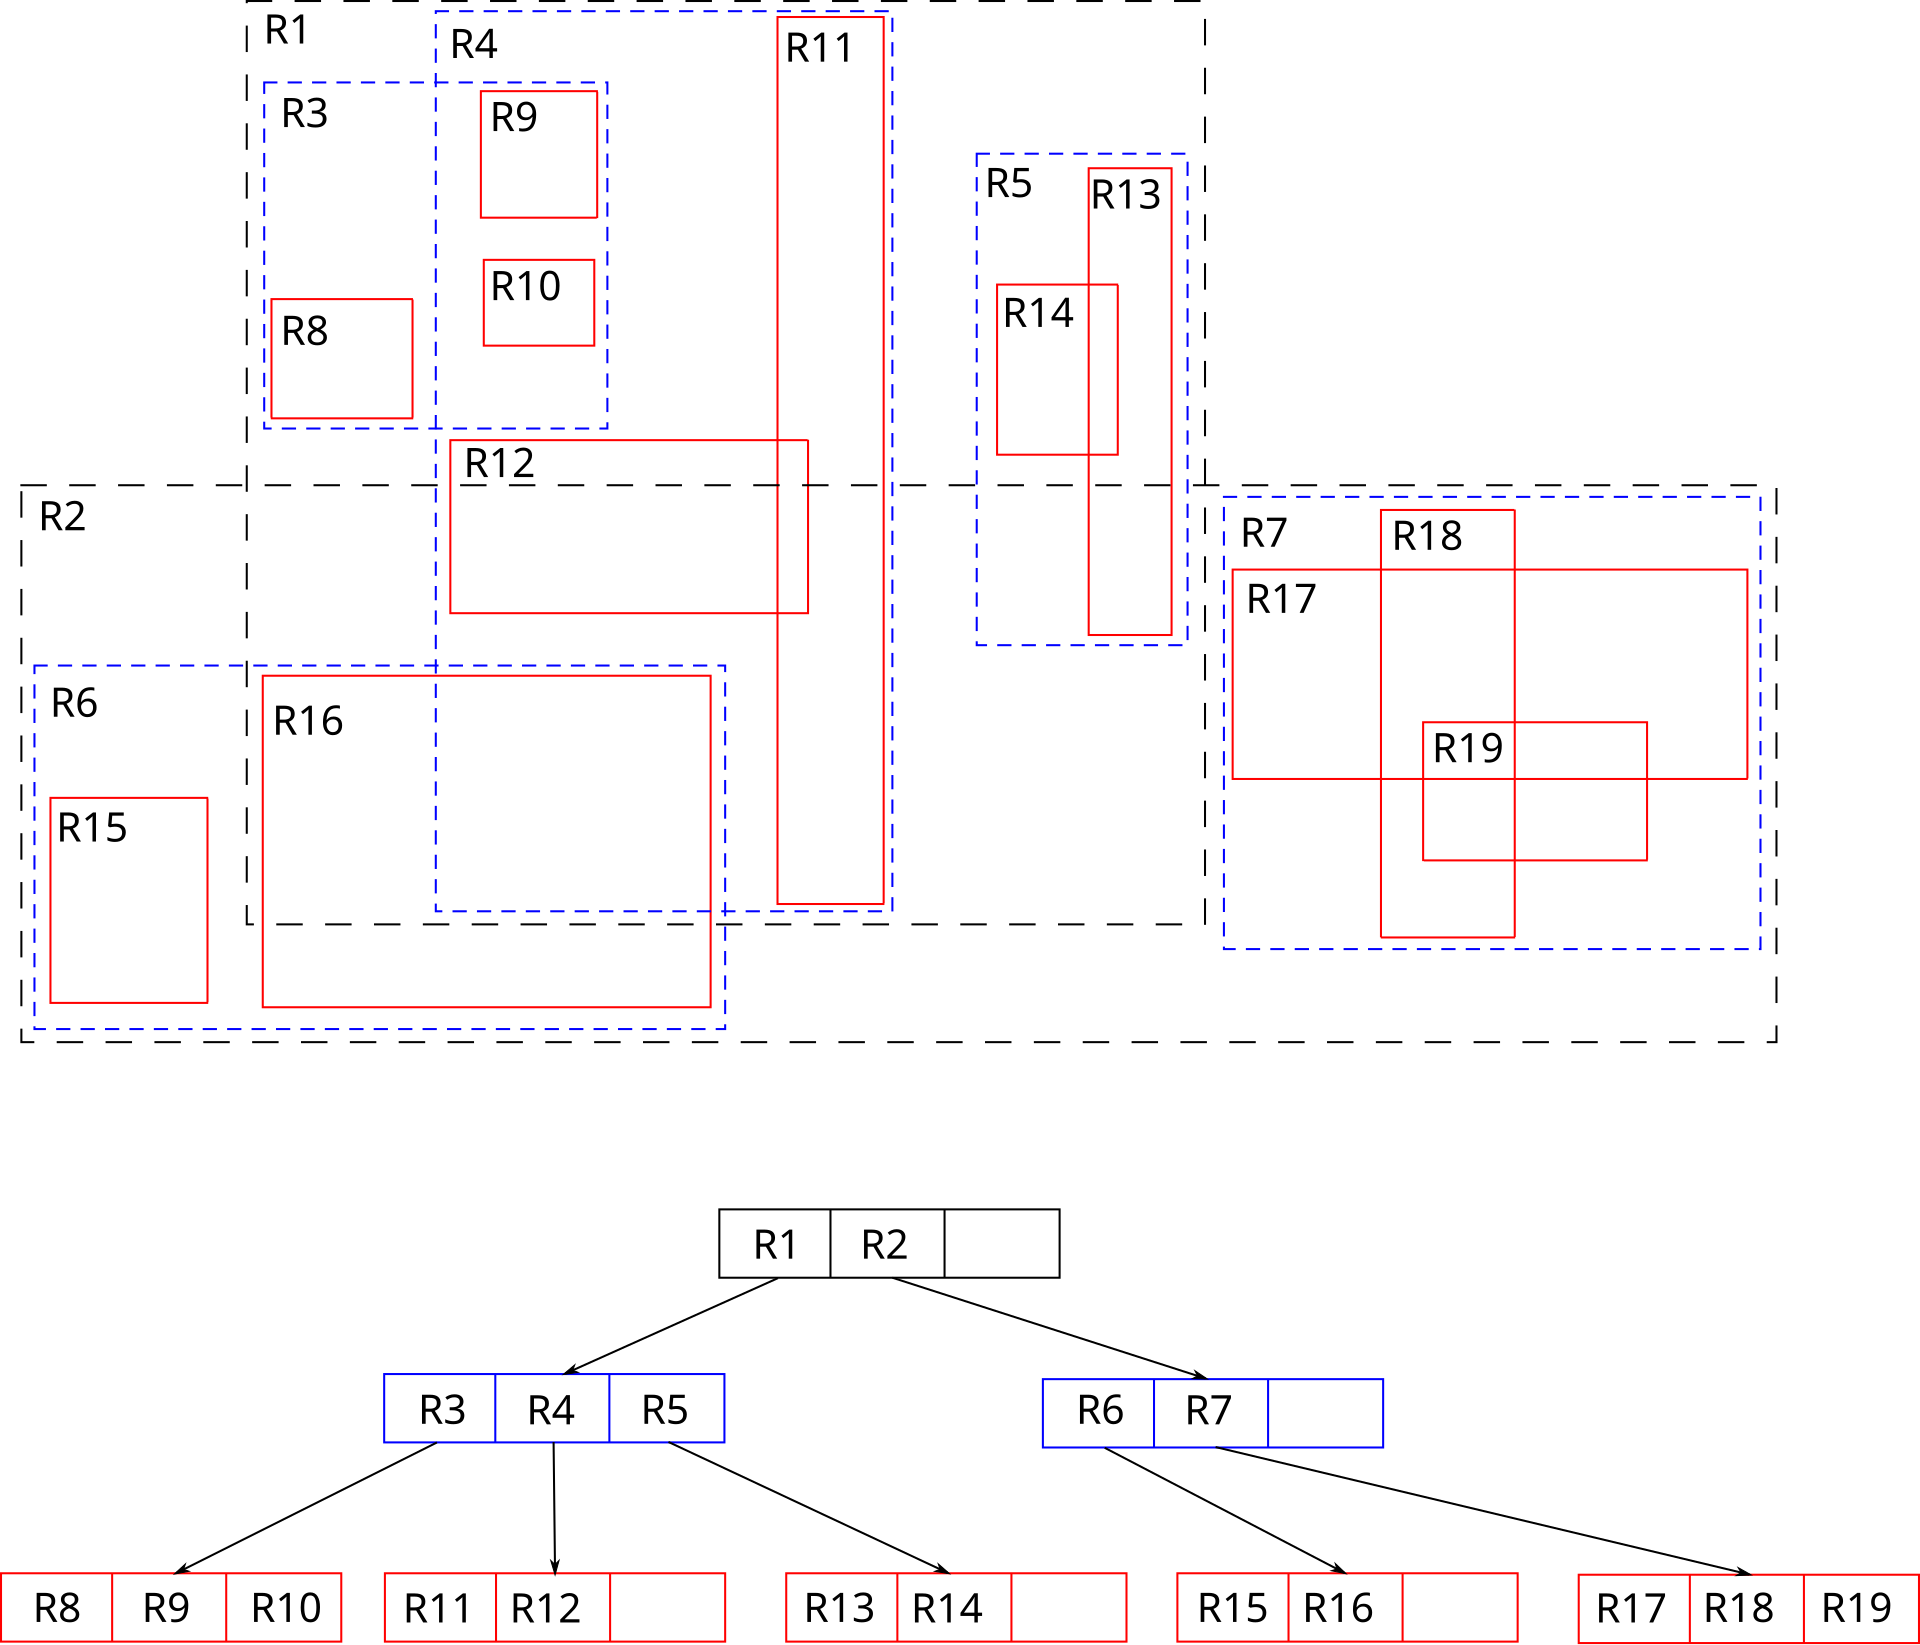
\includegraphics[width=\textwidth]{pic/2drtree.png}
	\caption{A simple R-Tree of 2D data}
\end{figure}

\subsection{Basic implementation and operations}
We begin with the first fundamental operation for R-Tree, that is the search algorithm. To be more specific, the \textbf{SEARCH} algorithm returns an array of all nodes whose MBRs overlap with the query MBR.
\begin{algorithm}{SEARCH \cite{Guttman1984}}
	\begin{enumerate}
		\item If the root is not a leaf node, for each entry, check whether their MBR overlap the searching MBR. For each satisfied node, call \textbf{SEARCH} on the corresponding subtree.
		\item If the root is a leaf node, for each entry, check whether their MBR overlap the searching MBR. Those that satisfied the condition belong to the result.
	\end{enumerate}
\end{algorithm}

We now describe the operation of splitting nodes in an R-Tree. Let $M$ be the largest number of children and $m\le M/2$ be the smallest number of children a node can contain. When a node overflows, that is, has more than $M$ children, the operation \textbf{SPLITNODE} is invoked. Here we will describe the linear splitting algorithm, which offers computational affordability but suboptimal query performance. We will now define a helper operation.
\begin{algorithm}{PICKSEEDS \cite{Guttman1984}}
	\begin{enumerate}
		\item Along each dimension, choose the node whose MBR has the highest low side and lowest high side and record their difference gap.
		\item Divide the width of the recorded set along the corresponding dimension, effectively normalizing the gaps.
		\item Select the pair with the greatest gap on any dimension.
	\end{enumerate}
\end{algorithm}

Now we are ready to define the operation \textbf{SPLITNODE}.

\begin{algorithm}{SPLITNODE \cite{Guttman1984}}
	\begin{enumerate}
		\item Invoke \textbf{PICKSEEDS} to choose 2 entries as the first element of each child node.
		\item If all entries have been selected, stop. If one child node has below $m$ entries, assign other entries to it and stop.
		\item Choose the next entry to assign and add it to the child node with least enlarged MBR requirement. Repeat step 2.
	\end{enumerate}
\end{algorithm}

The algorithm \textbf{ADJUSTTREE} updates MBRs by propagating from a leaf node to the root and performing node splits if necessary.

\begin{algorithm}{ADJUSTTREE \cite{Guttman1984}}
	\begin{enumerate}
		\item Let \textit{cur} be a copy of the query leaf node. If the query was previously split, let \textit{cur2} be a copy of the second leaf node.
		\item If \textit{cur} is the root, stop.
		\item Let \textit{parent} be the parent of \textit{cur}. Adjust the \textit{parent}'s corresponding entry's MBR to suit the MBRs of \textit{cur}.
		\item Do the same to \textit{cur2} using \textit{parent2}. Add its entry's MBR to the \textit{parent2}, in case of overfull, invoke \textbf{SPLITNODE} to produce two nodes to accommodate the children.
		\item Set \textit{cur} = \textit{parent} and \textit{cur2} = \textit{parent2}. Repeat from step 2.
	\end{enumerate}
\end{algorithm}

We are now ready to define our second fundamental operation, that is the \textbf{INSERT} operation.

\begin{algorithm}{INSERT \cite{Guttman1984}}
	\begin{enumerate}
		\item Let \textit{cur} be the root node.
		\item If \textit{cur} is a leaf node, skip to step 4.
		\item Set \textit{cur} to the child node whose MBR requires smallest enlargement to accommodate the new entry's MBR. If multiple are found, choose one with smallest area. Repeat from step 2.
		\item If \textit{cur} does not overflow when a new node is inserted, do so and stop. Otherwise, invoke \textbf{SPLITNODE} to accommodate the new node.
		\item Invoke \textbf{ADJUSTTREE} on \textit{cur}.
		\item If the root is split, set a new root whose children are the product of the split root.
	\end{enumerate}
\end{algorithm}

We now turn to our third and final fundamental operation, which is deleting a node from a tree. As per usual, we will define some helper operations to simplify the implementation. The operation \textbf{FINDLEAF} returns the leaf node containing the query node.

\begin{algorithm}{FINDLEAF \cite{Guttman1984}}
	\begin{enumerate}
		\item If the query node is a leaf node, check each entry of the node. If a match is found, return it.
		\item Otherwise, check each entry of the node whether their MBRs overlap the query MBR. For each matching node, invoke \textbf{FINDLEAF} on them.
	\end{enumerate}
\end{algorithm}

The operation \textbf{CONDENSETREE} is similar to \textbf{ADJUSTTREE} in that it reconfigures the tree after modifying the entries, i.e. deletion in the former and insertion in the latter.

\begin{algorithm}{CONDENSETREE \cite{Guttman1984}}
	\begin{enumerate}
		\item Let \textit{cur} be the query leaf node. Let \textit{deleted} be an array of deleted nodes.
		\item If \textit{cur} is the root, skip to step 6. Otherwise, let \textit{parent} be the parent node of \textit{cur}.
		\item If \textit{cur} underflows, delete its corresponding entries and append \textit{cur} to \textit{deleted}.
		\item If \textit{cur} is not deleted, adjust its MBR.
		\item Set \textit{cur} to \textit{parent} and repeat from step 2.
		\item Re-insert all entries from \textit{deleted}.
	\end{enumerate}
\end{algorithm}

We are now ready to define the operation \textbf{DELETE}.
\begin{algorithm}{DELETE \cite{Guttman1984}}
	\begin{enumerate}
		\item Invoke \textbf{FINDLEAF} to locate the query node. If none is found, stop.
		\item Remove the entry from the leaf node.
		\item Invoke \textbf{CONDENSETREE} on the leaf node.
		\item If the root node has only one child after tree condensation, make the child the new root.
	\end{enumerate}
\end{algorithm}

\subsection{C++ implementation}
\begin{lstlisting}[language=c++]
	// RTree.h

	#ifndef TREE_H
	#define TREE_H

	#include <vector>

	struct MBR {
		int x_min, y_min, x_max, y_max;
		MBR();
		MBR(int x_min, int y_min, int x_max, int y_max);
		int area() const;
		MBR merge(const MBR& other) const;
		bool contains(const MBR& other) const;
		bool intersects(const MBR& other) const;
	};

	struct Node {
		bool is_leaf;
		MBR mbr;
		std::vector<Node*> children;
		Node(bool is_leaf = false);
	};

	struct RTree {
		Node* root;
		int max_children;

		RTree(int max_children = 4);
		~RTree();
		void insert(const MBR& mbr);
		void search(const MBR& search_mbr);
		void find_area();
		void display_tree();

	private:
		void insert_recursive(Node* node, const MBR& mbr, Node* parent = nullptr);
		Node* choose_best_node(Node* node, const MBR& mbr);
		void split_node(Node* node, Node* parent);
		void update_mbr(Node* node);
		void search_recursive(Node* node, const MBR& search_mbr, std::vector<Node*>& results);
		void find_area_recursive(Node* node, int level);
		void delete_node(Node* node);
		void display_tree_recursive(Node* node, int level = 0);
	};

	#endif
\end{lstlisting}

\begin{lstlisting}[language=c++]
	// RTree-functions.cpp

	#include <iostream>
	#include <algorithm>
	#include "RTree.h"

	MBR::MBR() : x_min(0), y_min(0), x_max(0), y_max(0) {}
	MBR::MBR(int x_min, int y_min, int x_max, int y_max) : x_min(x_min), y_min(y_min), x_max(x_max), y_max(y_max) {}
	int MBR::area() const { return (x_max - x_min) * (y_max - y_min); }
	MBR MBR::merge(const MBR& other) const {
		return MBR(std::min(x_min, other.x_min), std::min(y_min, other.y_min),
			std::max(x_max, other.x_max), std::max(y_max, other.y_max));
	}
	bool MBR::contains(const MBR& other) const {
		return x_min <= other.x_min && y_min <= other.y_min && x_max >= other.x_max && y_max >= other.y_max;
	}
	bool MBR::intersects(const MBR& other) const {
		return !(x_max < other.x_min || x_min > other.x_max || y_max < other.y_min || y_min > other.y_max);
	}

	// Node constructor
	Node::Node(bool is_leaf) : is_leaf(is_leaf) {}

	// RTree methods
	RTree::RTree(int max_children) : max_children(max_children) {
		root = new Node(true);
	}

	RTree::~RTree() {
		delete_node(root);
	}

	void RTree::delete_node(Node* node) {
		if (!node) return;
		for (Node* child : node->children) {
			delete_node(child);
		}
		delete node;
	}

	void RTree::insert(const MBR& mbr) {
		insert_recursive(root, mbr, nullptr);
	}

	void RTree::insert_recursive(Node* node, const MBR& mbr, Node* parent) {
		if (node->is_leaf) {
			if (node->children.size() < max_children) {
				Node* new_node = new Node(true);
				new_node->mbr = mbr;
				node->children.push_back(new_node);
				update_mbr(node);
				if (parent) update_mbr(parent);
			}
			else {
				if (!parent) { // Root case
					Node* new_parent = new Node(false);
					split_node(node, new_parent);
					root = new_parent;
					Node* target = choose_best_node(new_parent, mbr);
					insert_recursive(target, mbr, new_parent);
				}
				else { // Non-root case
					split_node(node, parent);
					Node* target = choose_best_node(parent, mbr);
					insert_recursive(target, mbr, parent);
				}
			}
		}
		else {
			Node* target = choose_best_node(node, mbr);
			insert_recursive(target, mbr, node);
		}
	}

	Node* RTree::choose_best_node(Node* node, const MBR& mbr) {
		if (node->children.empty()) return node;
		Node* best = node->children[0];
		int min_enlargement = (node->children[0]->mbr.merge(mbr)).area() - node->children[0]->mbr.area();
		for (size_t i = 1; i < node->children.size(); ++i) {
			int enlargement = (node->children[i]->mbr.merge(mbr)).area() - node->children[i]->mbr.area();
			if (enlargement < min_enlargement) {
				min_enlargement = enlargement;
				best = node->children[i];
			}
		}
		return best;
	}

	void RTree::split_node(Node* node, Node* parent) {
		int median = node->children.size() / 2;
		Node* new_node = new Node(node->is_leaf);

		new_node->children = std::vector<Node*>(node->children.begin() + median, node->children.end());
		node->children = std::vector<Node*>(node->children.begin(), node->children.begin() + median);

		update_mbr(node);
		update_mbr(new_node);

		if (parent->children.empty()) {
			parent->children.push_back(node);
			parent->children.push_back(new_node);
		}
		else {
			for (size_t i = 0; i < parent->children.size(); ++i) {
				if (parent->children[i] == node) {
					parent->children[i] = node;
					parent->children.insert(parent->children.begin() + i + 1, new_node);
					break;
				}
			}
		}
		update_mbr(parent);
	}

	void RTree::update_mbr(Node* node) {
		if (node->children.empty()) return;
		node->mbr = node->children[0]->mbr;
		for (size_t i = 1; i < node->children.size(); ++i) {
			node->mbr = node->mbr.merge(node->children[i]->mbr);
		}
	}

	void RTree::search(const MBR& search_mbr) {
		std::vector<Node*> results;
		search_recursive(root, search_mbr, results);
		if (results.empty()) {
			std::cout << "No MBR found in the search range." << std::endl;
		}
		else {
			for (const Node* node : results) {
				std::cout << "Found MBR: (" << node->mbr.x_min << ", " << node->mbr.y_min
					<< ", " << node->mbr.x_max << ", " << node->mbr.y_max << ")\n";
			}
		}
	}

	void RTree::search_recursive(Node* node, const MBR& search_mbr, std::vector<Node*>& results) {
		if (node->is_leaf) {
			for (Node* child : node->children) {
				if (child->mbr.intersects(search_mbr)) {
					results.push_back(child);
				}
			}
		}
		else {
			for (Node* child : node->children) {
				if (child->mbr.intersects(search_mbr)) {
					search_recursive(child, search_mbr, results);
				}
			}
		}
	}

	void RTree::find_area() {
		if (root->children.empty()) {
			std::cout << "Tree is empty." << std::endl;
			return;
		}
		std::cout << "Areas of all MBRs in the R-tree:\n";
		find_area_recursive(root, 0);
	}

	void RTree::find_area_recursive(Node* node, int level) {
		std::string indent(level * 2, ' '); // Indentation based on level

		// Print the current node's MBR area
		std::cout << indent << (node->is_leaf ? "Leaf" : "Internal") << " Node MBR ("
			<< node->mbr.x_min << ", " << node->mbr.y_min << ", "
			<< node->mbr.x_max << ", " << node->mbr.y_max << "): "
			<< node->mbr.area() << std::endl;

		// If leaf, print areas of all child MBRs
		if (node->is_leaf) {
			for (size_t i = 0; i < node->children.size(); ++i) {
				Node* child = node->children[i];
				std::cout << indent << "  Child " << i + 1 << " MBR ("
					<< child->mbr.x_min << ", " << child->mbr.y_min << ", "
					<< child->mbr.x_max << ", " << child->mbr.y_max << "): "
					<< child->mbr.area() << std::endl;
			}
		}
		// If internal, recurse into children
		else {
			for (Node* child : node->children) {
				find_area_recursive(child, level + 1);
			}
		}
	}

	void RTree::display_tree() {
		if (root->children.empty()) {
			std::cout << "Tree is empty." << std::endl;
			return;
		}
		std::cout << "R-tree Structure:\n";
		display_tree_recursive(root, 0);
	}

	void RTree::display_tree_recursive(Node* node, int level) {
		if (!node) return;

		// Indentation based on depth
		for (int i = 0; i < level; ++i) {
			std::cout << "  ";
		}

		// Print the node's MBR
		std::cout << "|-- MBR (" << node->mbr.x_min << ", " << node->mbr.y_min
				<< ") to (" << node->mbr.x_max << ", " << node->mbr.y_max << ")";

		if (node->is_leaf) {
			std::cout << " [Leaf]";
		} else {
			std::cout << " [Internal]";
		}
		std::cout << std::endl;

		// Recursively print children
		for (Node* child : node->children) {
			display_tree_recursive(child, level + 1);
		}
	}
\end{lstlisting}

\subsection{Analysis}
Let $m$ and $n$ be the minimum number of children a node can contain and the number of nodes in the tree respectively. The operation \textbf{SEARCH} has a worst time complexity of $\Theta(n)$, where all nodes must be traversed. In the best case where there are no overlap, the best time complexity is $\Omega(\log_m n)$. One can observe that the average time complexity depends on the degree of overlapping nodes; that is, the node splitting method. The space required to store MBRs is $O(n)$ and since utilize recursion, the worst case space complexity is $\Theta(n)$ due to recursion stack.

As shown in the implementation, the operation \textbf{PICKSEEDS} has a time complexity of $O(\log_m n)$. In the case where splitting is required, the operation \textbf{SPLITNODE} is invoked, taking $\Theta(m)$ time in the worst case. We conclude that the operation \textbf{INSERT} has a time complexity of $O(\log_m n)$ on average and $\Theta(m\log_m n)$ in the worst case. It also uses $O(n)$ space to store $n$ objects. In a similar line of reasoning, the operation \textbf{DELETE} also has a time complexity of $\Theta(m\log_m n)$ in the worst case and a space complexity of $O(n)$.

\subsection{Application}
The R-Tree has a myriad of applications in the real world. A couple of questions posed regarding this is finding the closest restaurants in one's current location, or locating which bus crossed a region at some time interval. This in turn has raised an emergence to additional variants of the R-Tree, including but not limited to:
\begin{itemize}
	\item R*-tree
	\item R$^+$-tree
	\item 2+3-tree
	\item RT-tree.
\end{itemize}

\section{Exercises}
We conclude this report with a handful of mental gymnastics for the readers.
\subsection{Quizzes}
\begin{question}{1. What is the primary purpose of an R-tree data structure?}
	\begin{enumerate}[(a)]
		\item To store one-dimensional numerical data.
		\item To manage multi-dimensional spatial data.
		\item To store text-based data.
		\item To perform fast searching on strings.
	\end{enumerate}
\end{question}
Answer: (b) To manage multi-dimensional spatial data.

\begin{question}{2. In an R-tree, the leaf nodes contain}
	\begin{enumerate}[(a)]
		\item only pointers to the child nodes.
		\item bounding boxes that cover regions.
		\item actual spatial data or references to them.
		\item pairs of keys and values.
	\end{enumerate}
\end{question}
Answer: (c) actual spatial data or references to them.

\begin{question}{3. What type of data is most commonly indexed using an R-tree?}
	\begin{enumerate}[(a)]
		\item Linear numerical data.
		\item Multi-dimensional spatial data (e.g., geographic coordinates, rectangles).
		\item Text strings.
		\item Time series data.
	\end{enumerate}
\end{question}
Answer: (b) Multi-dimensional spatial data (e.g., geographic coordinates, rectangles).

\begin{question}{4. Which of the following is a key characteristic of an R-tree?}
	\begin{enumerate}[(a)]
		\item It is always unbalanced.
		\item It can only handle one-dimensional data.
		\item It uses bounding boxes to represent groups of spatial objects.
		\item It stores data as linked lists.
	\end{enumerate}
\end{question}
Answer: (c) It uses bounding boxes to represent groups of spatial objects.

\begin{question}{1. Count MBRs in an R-Tree}

	\quad In R-Tree, a node’s MBR is the smallest axis-aligned rectangle that encloses all the data points or sub-regions within that node.

	\quad Given a root of an R-Tree, you are asked to return the total number of MBRs.

	\quad \underline{Constraint}: The R-Tree has a maximum fanout (number of children per node) of 4, and you must count the total number of MBRs without using recursion (e.g., use an iterative approach like a stack or queue).
\end{question}

\begin{lstlisting}[language=c++]
	int RTree::count_mbrs() {
		return count_mbrs_recursive(root);
	}

	int RTree::count_mbrs_recursive(NOde* node) {
		if (!node) return 0;
		if (node->is_leaf) {
			return node->children.size(); //Leaf nodes store MBRs directly
		}
		int total=0;
		for (Node* child : node->children) {
			total += count_mbrs_recursive(child);
		}
		return total;
	}
\end{lstlisting}

\begin{question}{2. Find overlapping MBRs in a range}
	
	\quad Two MBRs are called overlapped when they enclose the same space in the tree.
	
	\quad Given a R-Tree, its root and a range (a rectangle with coordinates), you are asked to return the number of overlapping MBRs in that range, and coordinates of each MBR. 
	
	\quad \underline{Constraint}: The R-Tree contains at least 10,000 nodes, and you must optimize the solution to run in O(log n + k) time complexity, where k is the number of overlapping MBRs, assuming a balanced R-Tree.
\end{question}

\begin{lstlisting}[language=c++]
	void RTree::count_overlaps(const MBR& range) {
		std::vector<Node*> overlaps;
		search_recursive(root, range, overlaps);
		std::cout << "Number of MBRs overlapping with (" << range.x_min << ", " << range.y_min << ", " << range.x_max << ", " << range.y_max << "): " << overlaps.size() << std::endl;
		for (const Node* node : overlaps) {
			std::cout << "  Overlapping MBR: (" << node->mbr.x_min << ", " << node->mbr.y_min << ", " << node->mbr.x_max << ", " << node->mbr.y_max << ")\n";
		}
	}
\end{lstlisting}

\begin{question}{3. Calculate total area covered}
	
	\quad Each MBR in R-Tree represent a region which have its own area. Due to overlapping effect, there is a difference in root's MBR and all-leaves' MBRs.

	\quad Given a R-Tree and its root, you are asked to calculate the sum of all leaf-level-MBRs' area and a area of root's MBR.

	\quad \underline{Constraint}: The coordinates of the MBRs may include floating-point values, and you must compute the areas with a precision of at least 6 decimal places, accounting for potential numerical errors.
\end{question}

\begin{lstlisting}[language=c++]
	void RTree::total_area() {
		if (root->children.empty()) {
			std::cout << "Tree is empty. Root area: 0, Total leaf area: 0" << std::endl;
			return;
		}
		int root_area = root->mbr.area();
		int leaf_total = total_area_recursive(root);
		std::cout << "Root MBR Area (" << root->mbr.x_min << ", " << root->mbr.y_min << ", " << root->mbr.x_max << ", " << root->mbr.y_max << "): " << root_area << std::endl;
		std::cout << "Total Leaf MBR Area: " << leaf_total << std::endl;
	}

	int RTree::total_area_recursive(Node* node) {
		if (node->is_leaf) {
			int total = 0;
			for (Node* child : node->children) {
				total += child->mbr.area();
			}
			return total;
		}
		int total = 0;
		for (Node* child : node->children) {
			total += total_area_recursive(child);
		}
		return total;
	}
\end{lstlisting}

\printbibliography

\end{document}